\documentclass[tikz,border=4mm]{standalone}

\usepackage[T1]{fontenc}
\usepackage{amsmath,amssymb,bm}
\usepackage{newtxtext,newtxmath}
\usetikzlibrary{arrows.meta,calc,positioning}

\definecolor{ink}{HTML}{1F2A44}
\definecolor{accent}{HTML}{9A3B2F}
\definecolor{sea}{HTML}{2E6E6B}
\definecolor{sand}{HTML}{F2EEE6}
\definecolor{ash}{HTML}{6B7280}

\newcommand{\KL}{\mathrm{KL}}
\newcommand{\E}{\mathbb{E}}
\newcommand{\xx}{\bm{x}}
\newcommand{\dd}{\mathop{}\!\mathrm{d}}

\begin{document}
% Exact source of figures/04-kl-wasserstein-flow.tex from the book.
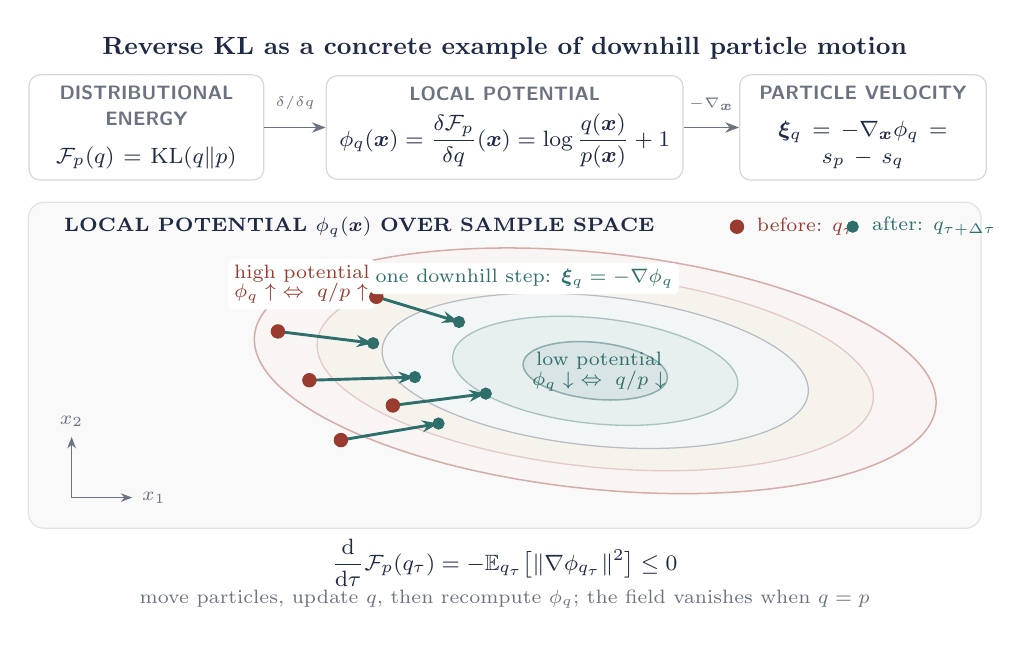
\begin{tikzpicture}[
  >=Stealth,
  font=\footnotesize,
  particle/.style={
    circle,
    draw=accent,
    fill=accent,
    minimum size=4.8pt,
    inner sep=0pt
  },
  moved/.style={
    circle,
    draw=sea,
    fill=sea,
    minimum size=4pt,
    inner sep=0pt
  },
  descent/.style={
    sea,
    line width=1.05pt,
    -{Stealth[length=2.1mm,width=1.5mm]}
  },
  stepbox/.style={
    rounded corners=1.4mm,
    draw=ash!28,
    fill=white,
    line width=.45pt,
    minimum height=1.10cm,
    inner sep=4pt,
    align=center
  }
]

\node[font=\bfseries\small,color=ink]
  at (6.30,7.18)
  {Reverse KL as a concrete example of downhill particle motion};

\node[stepbox,text width=2.70cm] (energy) at (1.75,6.17) {%
  {\color{ash}\sffamily\fontsize{6.6}{7.5}\selectfont\bfseries
   DISTRIBUTIONAL ENERGY}\\[4pt]
  {\color{ink}$\displaystyle\mathcal F_p(q)=\KL(q\|p)$}};

\node[stepbox,text width=4.25cm] (potential) at (6.30,6.17) {%
  {\color{ash}\sffamily\fontsize{6.6}{7.5}\selectfont\bfseries
   LOCAL POTENTIAL}\\[4pt]
  {\color{ink}$\displaystyle
    \phi_q(\xx)
    =\frac{\delta\mathcal F_p}{\delta q}(\xx)
    =\log\frac{q(\xx)}{p(\xx)}+1$}};

\node[stepbox,text width=2.85cm] (velocity) at (10.85,6.17) {%
  {\color{ash}\sffamily\fontsize{6.6}{7.5}\selectfont\bfseries
   PARTICLE VELOCITY}\\[4pt]
  {\color{ink}$\displaystyle
    \bm\xi_q=-\nabla_{\xx}\phi_q=s_p-s_q$}};

\draw[ash,line width=.65pt,-{Stealth[length=1.75mm]}]
  (energy.east) -- (potential.west)
  node[midway,above=2.5pt,text=ash,font=\tiny]
  {$\delta/\delta q$};
\draw[ash,line width=.65pt,-{Stealth[length=1.75mm]}]
  (potential.east) -- (velocity.west)
  node[midway,above=2.5pt,text=ash,font=\tiny]
  {$-\nabla_{\xx}$};

\path[rounded corners=2mm,fill=ash!4,draw=ash!20,line width=.45pt]
  (.25,1.08) rectangle (12.35,5.22);

\node[anchor=west,color=ink,font=\scriptsize\bfseries]
  at (.58,4.91) {LOCAL POTENTIAL $\phi_q(\xx)$ OVER SAMPLE SPACE};

\node[particle] at (9.25,4.91) {};
\node[anchor=west,color=accent,font=\scriptsize]
  at (9.38,4.91) {before: $q_\tau$};
\node[moved] at (10.72,4.91) {};
\node[anchor=west,color=sea,font=\scriptsize]
  at (10.84,4.91) {after: $q_{\tau+\Delta\tau}$};

\begin{scope}[shift={(7.45,3.08)},rotate=-6]
  \fill[accent!5] (0,0) ellipse [x radius=4.35,y radius=1.50];
  \fill[sand!72]  (0,0) ellipse [x radius=3.55,y radius=1.22];
  \fill[sea!6]    (0,0) ellipse [x radius=2.72,y radius=.95];
  \fill[sea!11]   (0,0) ellipse [x radius=1.82,y radius=.67];
  \fill[sea!18]   (0,0) ellipse [x radius=.92,y radius=.36];

  \draw[accent!42,line width=.55pt]
    (0,0) ellipse [x radius=4.35,y radius=1.50];
  \draw[accent!27,line width=.48pt]
    (0,0) ellipse [x radius=3.55,y radius=1.22];
  \draw[ash!48,line width=.45pt]
    (0,0) ellipse [x radius=2.72,y radius=.95];
  \draw[sea!42,line width=.48pt]
    (0,0) ellipse [x radius=1.82,y radius=.67];
  \draw[sea!55,line width=.55pt]
    (0,0) ellipse [x radius=.92,y radius=.36];
\end{scope}

\node[anchor=west,color=accent,font=\scriptsize,align=left,
      fill=white,rounded corners=.8mm,inner sep=2.2pt]
  at (2.78,4.18)
  {high potential\\[-1pt] $\phi_q\uparrow\;\Leftrightarrow\;q/p\uparrow$};
\node[anchor=center,color=sea,font=\scriptsize,align=center]
  at (7.50,3.07)
  {low potential\\[-1pt] $\phi_q\downarrow\;\Leftrightarrow\;q/p\downarrow$};

\coordinate (p1) at (3.42,3.58);
\coordinate (p2) at (3.82,2.96);
\coordinate (p3) at (4.22,2.20);
\coordinate (p4) at (4.67,4.02);
\coordinate (p5) at (4.88,2.64);

\coordinate (r1) at (4.63,3.43);
\coordinate (r2) at (5.16,3.00);
\coordinate (r3) at (5.46,2.41);
\coordinate (r4) at (5.72,3.70);
\coordinate (r5) at (6.06,2.79);

\draw[descent] (p1) -- (r1);
\draw[descent] (p2) -- (r2);
\draw[descent] (p3) -- (r3);
\draw[descent] (p4) -- (r4);
\draw[descent] (p5) -- (r5);

\foreach \p in {p1,p2,p3,p4,p5} {
  \node[particle] at (\p) {};
}
\foreach \p in {r1,r2,r3,r4,r5} {
  \node[moved] at (\p) {};
}

\node[anchor=center,color=sea,font=\scriptsize,
      fill=white,rounded corners=.8mm,inner sep=2.2pt]
  at (6.55,4.25)
  {one downhill step: $\bm\xi_q=-\nabla\phi_q$};

\draw[ash,line width=.55pt,-{Stealth[length=1.45mm]}]
  (.80,1.47) -- (1.57,1.47)
  node[right,color=ash,font=\scriptsize] {$x_1$};
\draw[ash,line width=.55pt,-{Stealth[length=1.45mm]}]
  (.80,1.47) -- (.80,2.24)
  node[above,color=ash,font=\scriptsize] {$x_2$};

\node[color=ink] at (6.30,.64)
  {$\displaystyle
    \frac{\dd}{\dd\tau}\mathcal F_p(q_\tau)
    =-\E_{q_\tau}
       \bigl[\|\nabla\phi_{q_\tau}\|^2\bigr]\leq0$};
\node[color=ash,font=\scriptsize] at (6.30,.18)
  {move particles, update $q$, then recompute $\phi_q$;
   the field vanishes when $q=p$};

\end{tikzpicture}
\end{document}
